\documentclass{article}


% if you need to pass options to natbib, use, e.g.:
%     \PassOptionsToPackage{numbers, compress}{natbib}
% before loading neurips_2023


% ready for submission
\usepackage{neurips_2023}


% to compile a preprint version, e.g., for submission to arXiv, add add the
% [preprint] option:
% \usepackage[preprint]{neurips_2023}


% to compile a camera-ready version, add the [final] option, e.g.:
%     \usepackage[final]{neurips_2023}


% to avoid loading the natbib package, add option nonatbib:
%    \usepackage[nonatbib]{neurips_2023}


\usepackage[utf8]{inputenc} % allow utf-8 input
\usepackage[T1]{fontenc}    % use 8-bit T1 fonts
\usepackage{hyperref}       % hyperlinks
\usepackage{url}            % simple URL typesetting
\usepackage{booktabs}       % professional-quality tables
\usepackage{amsfonts}       % blackboard math symbols
\usepackage{nicefrac}       % compact symbols for 1/2, etc.
\usepackage{microtype}      % microtypography
\usepackage{xcolor}         % colors

\usepackage{amsmath}
\usepackage{amsthm}
\usepackage{caption}
\usepackage{graphicx}
\usepackage{algorithm}
\usepackage{algpseudocode}
\usepackage{import}
\usepackage{booktabs}
\usepackage{longtable}
\usepackage{array}
\usepackage{multirow}

% Bibliography
\bibliographystyle{plainnat}
\setcitestyle{numbers,square,comma}

% Numbered Environments:
\newtheorem{definition}{Definition}[section]
\newtheorem{question}{Research Question}[section]


\title{ECCCos from the Black Box:\\
Faithful Explanations through\\
Energy-Constrained Conformal Counterfactuals}


% The \author macro works with any number of authors. There are two commands
% used to separate the names and addresses of multiple authors: \And and \AND.
%
% Using \And between authors leaves it to LaTeX to determine where to break the
% lines. Using \AND forces a line break at that point. So, if LaTeX puts 3 of 4
% authors names on the first line, and the last on the second line, try using
% \AND instead of \And before the third author name.


\author{%
  Patrick Altmeyer\thanks{Use footnote for providing further information
    about author (webpage, alternative address)---\emph{not} for acknowledging
    funding agencies.} \\
  Faculty of Electrical Engineering, Mathematics and Computer Science\\
  Delft University of Technology\\
  2628 XE Delft, The Netherlands \\
  \texttt{p.altmeyer@tudelft.nl} \\
  % examples of more authors
  % \And
  % Coauthor \\
  % Affiliation \\
  % Address \\
  % \texttt{email} \\
  % \AND
  % Coauthor \\
  % Affiliation \\
  % Address \\
  % \texttt{email} \\
  % \And
  % Coauthor \\
  % Affiliation \\
  % Address \\
  % \texttt{email} \\
  % \And
  % Coauthor \\
  % Affiliation \\
  % Address \\
  % \texttt{email} \\
}


\begin{document}


\maketitle


\begin{abstract}
  Counterfactual Explanations offer an intuitive and straightforward way to explain black-box models and offer Algorithmic Recourse to individuals. To address the need for plausible explanations, existing work has primarily relied on surrogate models to learn how the input data is distributed. This effectively reallocates the task of learning realistic explanations for the data from the model itself to the surrogate. Consequently, the generated explanations may seem plausible to humans but need not necessarily describe the behaviour of the black-box model faithfully. We formalise this notion of faithfulness through the introduction of a tailored evaluation metric and propose a novel algorithmic framework for generating \textbf{E}nergy-\textbf{C}onstrained \textbf{C}onformal \textbf{Co}unterfactuals (ECCCos) that are only as plausible as the model permits. Through extensive empirical studies involving multiple synthetic and real-world datasets, we demonstrate that ECCCos reconcile the need for plausibility and faithfulness. In particular, we show that it is possible to achieve state-of-the-art plausibility for models with gradient access without the need for surrogate models. To do so, our framework relies solely on properties defining the black-box model itself by leveraging recent advances in energy-based modelling and conformal prediction. To our knowledge, this is the first venture in this direction for generating faithful Counterfactual Explanations. Thus, we anticipate that ECCCos can serve as a baseline for future research. We believe that our work opens avenues for researchers and practitioners seeking tools to better distinguish trustworthy from unreliable models.
\end{abstract}

\section{Introduction}\label{intro}

Counterfactual Explanations (CE) provide a powerful, flexible and intuitive way to not only explain black-box models but also help affected individuals through the means of Algorithmic Recourse. Instead of opening the Black Box, CE works under the premise of strategically perturbing model inputs to understand model behaviour~\citep{wachter2017counterfactual}. Intuitively speaking, we generate explanations in this context by asking what-if questions of the following nature: `Our credit risk model currently predicts that this individual is not credit-worthy. What if they reduced their monthly expenditures by 10\%?'

This is typically implemented by defining a target outcome $\mathbf{y}^+ \in \mathcal{Y}$ for some individual $\mathbf{x} \in \mathcal{X}=\mathbb{R}^D$ described by $D$ attributes, for which the model $M_{\theta}:\mathcal{X}\mapsto\mathcal{Y}$ initially predicts a different outcome: $M_{\theta}(\mathbf{x})\ne \mathbf{y}^+$. Counterfactuals are then searched by minimizing a loss function that compares the predicted model output to the target outcome: $\text{yloss}(M_{\theta}(\mathbf{x}),\mathbf{y}^+)$. Since Counterfactual Explanations work directly with the black-box model, valid counterfactuals always have full local fidelity by construction where fidelity is defined as the degree to which explanations approximate the predictions of a black-box model~\citep{mothilal2020explaining,molnar2020interpretable}. 

In situations where full fidelity is a requirement, CE offers a more appropriate solution to Explainable Artificial Intelligence (XAI) than other popular approaches like LIME~\citep{ribeiro2016why} and SHAP~\citep{lundberg2017unified}, which involve local surrogate models. But even full fidelity is not a sufficient condition for ensuring that an explanation faithfully describes the behaviour of a model. That is because multiple very distinct explanations can all lead to the same model prediction, especially when dealing with heavily parameterized models like deep neural networks, which are typically underspecified by the data~\citep{wilson2020case}.

In the context of CE, the idea that no two explanations are the same arises almost naturally. A key focus in the literature has therefore been to identify those explanations and algorithmic recourses that are most appropriate based on a myriad of desiderata such as sparsity, actionability and plausibility. In this work, we draw closer attention to model faithfulness rather than fidelity as a desideratum for counterfactuals. Our key contributions are as follows: 

\begin{itemize}
  \item We demonstrate that a narrow focus on plausibility can yield counterfactuals that are unfaithful to model behaviour despite having full fidelity (Section~\ref{fidelity}).
  \item We propose a definition of faithfulness that gives rise to a more suitable evaluation metric for counterfactuals than fidelity (Section~\ref{faithfulness}).
  \item We introduce a novel algorithmic approach for generating Energy-Constrained Conformal Counterfactuals (ECCCos) in Section~\ref{meth}.
  \item We provide extensive empirical evidence demonstrating that ECCCos faithfully explain model behaviour without sacrificing plausibility (Section~\ref{emp}).
\end{itemize}

Thus, we believe that our work opens avenues for researchers and practitioners seeking tools to better distinguish trustworthy from unreliable models.

\section{Background}\label{background}

While Counterfactual Explanations can be generated for arbitrary regression models~\citep{spooner2021counterfactual}, existing work has primarily focused on classification problems. Let $\mathcal{Y}=(0,1)^K$ denote the one-hot-encoded output domain with $K$ classes. Then most counterfactual generators rely on gradient descent to optimize different flavours of the following counterfactual search objective:

\begin{equation} \label{eq:general}
\begin{aligned}
\mathbf{Z}^\prime &= \arg \min_{\mathbf{Z}^\prime \in \mathcal{Z}^L} \left\{  {\text{yloss}(M_{\theta}(f(\mathbf{Z}^\prime)),\mathbf{y}^+)}+ \lambda {\text{cost}(f(\mathbf{Z}^\prime)) }  \right\} 
\end{aligned} 
\end{equation}

Here $\text{yloss}$ denotes the primary loss function already introduced above and $\text{cost}$ is either a single penalty or a collection of penalties that are used to impose constraints through regularization. Equation~\ref{eq:general} restates the baseline approach to gradient-based counterfactual search proposed by~\citet{wachter2017counterfactual} in general form where $\mathbf{Z}^\prime=\{ \mathbf{z}_l\}_L$ denotes an $L$-dimensional array of counterfactual states~\citep{altmeyer2023endogenous}. This is to explicitly account for the multiplicity of explanations and the fact that we may choose to generate multiple counterfactuals and traverse a latent encoding $\mathcal{Z}$ of the feature space $\mathcal{X}$ where we denote $f^{-1}: \mathcal{X} \mapsto \mathcal{Z}$. Encodings may involve simple feature transformations or more advanced techniques involving generative models, as we will discuss further below. The baseline approach, which we will simply refer to as \textbf{Wachter}~\citep{wachter2017counterfactual}, searches a single counterfactual directly in the feature space and penalises its distance to the original factual. 
\section{Why Fidelity is not Enough}\label{fidelity}

Counterfactual Explanations have full fidelity by construction as long as they are valid. Solutions to Equation~\ref{eq:general} are considered valid as soon as the predicted label matches the target label. A stripped-down counterfactual explanation is therefore little different from an adversarial example. In Figure~\ref{fig:adv}, for example, we have applied Wachter to MNIST data (centre panel) where the underlying classifier $M_{\theta}$ is a simple Multi-Layer Perceptron (MLP) with above 90 percent test accuracy. For the generated counterfactual $\mathbf{x}^{\prime}$ the model predicts the target label with high confidence (centre panel in Figure~\ref{fig:adv}). The explanation is valid by definition and therefore has full fidelity, even though it looks a lot like an Adversarial Example~\citep{goodfellow2014explaining}. \citet{schut2021generating} make the connection between Adversarial Examples and Counterfactual Explanations explicit and propose using a Jacobian-Based Saliency Map Attack (JSMA) to solve Equation~\ref{eq:general}. They demonstrate that this approach yields plausible counterfactuals for Bayesian, adversarially robust classifiers. Applying their approach to our simple MNIST classifier does not yield a realistic counterfactual but this one, too, is valid (right panel in Figure~\ref{fig:adv}). 

\begin{figure}
  \centering
  \begin{minipage}[t]{0.45\textwidth}
    \centering
    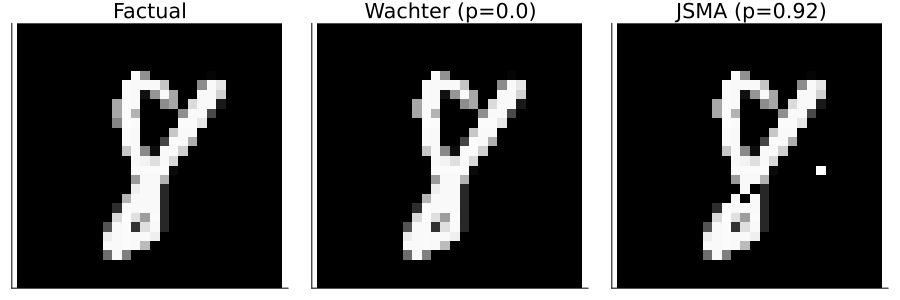
\includegraphics[width=\textwidth]{../artifacts/results/images/you_may_not_like_it.png}
    \caption{Explanations or Adversarial Examples? Counterfactuals for turning a 9 (nine) into a 7 (seven): original image (left); counterfactual produced using~\citet{wachter2017counterfactual} (centre); and a counterfactual produced using the approach introduced by~\citep{schut2021generating} that uses Jacobian-Based Saliency Map Attacks to solve Equation~\ref{eq:general}.}\label{fig:adv}
  \end{minipage}\hfill
  \begin{minipage}[t]{0.45\textwidth}
    \centering
    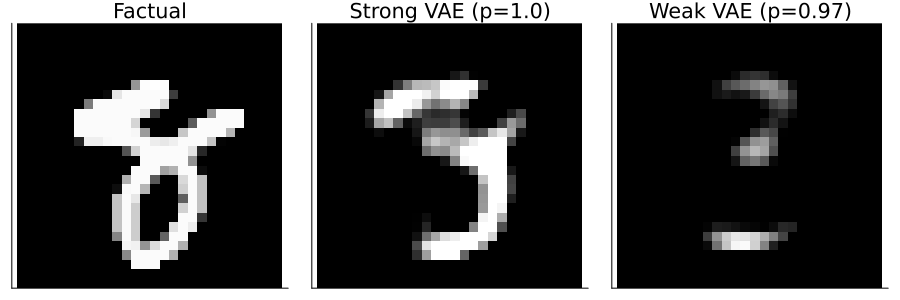
\includegraphics[width=\textwidth]{../artifacts/results/images/surrogate_gone_wrong.png}
    \caption{Using surrogates can improve plausibility, but also increases vulnerability. Counterfactuals for turning an 9 (nine) into a 7 (seven): original image (left); counterfactual produced using REVISE~\citep{joshi2019realistic} with a well-specified surrogate (centre); and a counterfactual produced using REVISE~\citep{joshi2019realistic} with a poorly specified surrogate (right).}\label{fig:vae}
  \end{minipage}
\end{figure}

The crucial difference between Adversarial Examples (AE) and Counterfactual Explanations is one of intent. While an AE is intended to go unnoticed, a CE should have certain desirable properties. The literature has made this explicit by introducing various so-called \textit{desiderata} that counterfactuals should meet in order to properly serve both AI practitioners and individuals affected by AI decision-making systems. The list of desiderate includes but is not limited to the following: sparsity, proximity~\citep{wachter2017counterfactual}, actionability~\citep{ustun2019actionable}, diversity~\citep{mothilal2020explaining}, plausibility~\citep{joshi2019realistic,poyiadzi2020face,schut2021generating}, robustness~\citep{upadhyay2021robust,pawelczyk2022probabilistically,altmeyer2023endogenous} and causality~\citep{karimi2021algorithmic}.

Researchers have come up with various ways to meet these desiderata, which have been extensively surveyed and evaluated in various studies~\citep{verma2020counterfactual,karimi2020survey,pawelczyk2021carla,artelt2021evaluating,guidotti2022counterfactual}. Perhaps unsurprisingly, the different desiderata are often positively correlated. For example, \citet{artelt2021evaluating} find that plausibility typically also leads to improved robustness. Similarly, plausibility has also been connected to causality in the sense that plausible counterfactuals respect causal relationships~\citep{mahajan2020preserving}. Consequently, the plausibility of counterfactuals has been among the primary concerns for researchers. 

Achieving plausibility is equivalent to ensuring that the generated counterfactuals comply with the true and unobserved data-generating process (DGP). Formally, this can be defined as follows:

\begin{definition}[Plausible Counterfactuals]
  \label{def:plausible}
  Let $\mathcal{X}|\mathbf{y}^+$ denote the true conditional distribution of samples in the target class $\mathbf{y}^+$. Then for $\mathbf{x}^{\prime}$ to be considered a plausible counterfactual, we need: $\mathbf{x}^{\prime} \sim \mathcal{X}|\mathbf{y}^+$.
\end{definition}

To generate plausible counterfactuals, we need to be able to quantify the DGP: $\mathcal{X}|\mathbf{y}^+$. One straightforward way to do this is to use surrogate models for the task. \citet{joshi2019realistic}, for example, suggest that instead of searching counterfactuals in the feature space $\mathcal{X}$, we can instead traverse a latent embedding $\mathcal{Z}$ (Equation~\ref{eq:general}) that implicitly codifies the DGP. To learn the latent embedding, they propose using a generative model such as a Variational Autoencoder (VAE). Provided the surrogate model is well-trained, their proposed approach ---\textbf{REVISE}--- can yield plausible explanations like the one in the centre panel of Figure~\ref{fig:vae}. Others have proposed similar approaches: \citet{dombrowski2021diffeomorphic} traverse the base space of a normalizing flow to solve Equation~\ref{eq:general}; \citet{poyiadzi2020face} use density estimators ($\hat{p}: \mathcal{X} \mapsto [0,1]$) to constrain the counterfactuals to dense regions in the feature space; and, finally, \citet{karimi2021algorithmic} assume knowledge about the structural causal model that generates the data. 

While surrogates offer an easy way to address the need for plausibility, they also introduce friction: the generated explanations no longer depend exclusively on the black-box model itself. The counterfactual in the centre panel of Figure~\ref{fig:vae}, for example, looks more plausible than the corresponding counterfactuals generated by \textbf{Wachter} and \textbf{Schut}. But is it also more faithful to the behaviour of our MNIST classifier? Fidelity cannot help us to make that judgement, because all of these counterfactuals have full fidelity. To bridge this gap, we introduce a new notion of faithfulness in the following section.

\section{A new Notion of Faithfulness}\label{faithfulness}

Analogous to Definition~\ref{def:plausible}, we propose to define faithfulness in the context of Counterfactual Explanations as follows:

\begin{definition}[Faithful Counterfactuals]
  \label{def:faithful}
  Let $\mathcal{X}_{\theta}|\mathbf{y}^+ = p_{\theta}(\mathbf{X}_{\mathbf{y}^+})$ denote the conditional distribution of $\mathbf{x}$ in the target class $\mathbf{y}^+$, where $\theta$ denotes the parameters of model $M_{\theta}$. Then for $\mathbf{x}^{\prime}$ to be considered a conformal counterfactual, we need: $\mathbf{x}^{\prime} \sim \mathcal{X}_{\theta}|\mathbf{y}^+$.
\end{definition}

In doing this, we merge in and nuance the concept of plausibility (Definition~\ref{def:plausible}) where the notion of `consistent with the data' becomes `consistent with what the model has learned about the data'.

\subsection{Quantifying the Model's Generative Property}

To assess counterfactuals with respect to Definition~\ref{def:faithful}, we need a way to quantify the posterior conditional distribution $p_{\theta}(\mathbf{x}|\mathbf{y}^+)$. To this end, we draw on recent advances in Energy-Based Modelling (EBM), a subdomain of machine learning that is concerned with generative or hybrid modelling~\citep{grathwohl2020your,}. In particular, note that if we fix $\mathbf{y}$ to our target value $\mathbf{y}^+$, we can conditionally draw from $p_{\theta}(\mathbf{x}|\mathbf{y}^+)$ using Stochastic Gradient Langevin Dynamics (SGLD) as follows, 

\begin{equation}\label{eq:sgld}
  \begin{aligned}
    \mathbf{x}_{j+1} &\leftarrow \mathbf{x}_j - \frac{\epsilon^2}{2} \mathcal{E}(\mathbf{x}_j|\mathbf{y}^+) + \epsilon \mathbf{r}_j, && j=1,...,J
  \end{aligned}
\end{equation}

where $\mathbf{r}_j \sim \mathcal{N}(\mathbf{0},\mathbf{I})$ is the stochastic term and the step-size $\epsilon$ is typically polynomially decayed~\citep{welling2011bayesian}. The term $\mathcal{E}(\mathbf{x}_j|\mathbf{y}^+)$ denotes the model energy conditioned on the target class label $\mathbf{y}^+$. To allow for faster sampling, we follow the common practice of choosing the step-size $\epsilon$ and the standard deviation of $\mathbf{r}_j$ separately. While $\mathbf{x}_J$ is only guaranteed to distribute as $p_{\theta}(\mathbf{x}|\mathbf{y}^*)$ if $\epsilon \rightarrow 0$ and $J \rightarrow \infty$, the bias introduced for a small finite $\epsilon$ is negligible in practice \citep{murphy2023probabilistic,grathwohl2020your}. Appendix~\ref{app-jem} provides additional implementation details for any tasks related to energy-based modelling. 

Generating multiple samples using SGLD thus yields an empirical distribution $\hat{\mathbf{X}}_{\theta,\mathbf{y}^+}$ that approximates what the model has learned about the input data. While in the context of Energy-Based Modelling, this is usually done during training, we propose to use SGLD during inference in order to evaluate and generate faithful model explanations.

\subsection{Evaluating Plausibility and Faithfulness}

The parallels between our definitions of plausibility and faithfulness imply that we can also use similar evaluation metrics in both cases. Since existing work has focused heavily on plausibility, it offers a useful starting point. In particular,~\citet{guidotti2022counterfactual} have proposed an implausibility metric that measures the distance of the counterfactual from its nearest neighbour in the target class. As this distance is reduced, counterfactuals get more plausible under the assumption that the nearest neighbour itself is plausible in the sense of Definition~\ref{def:plausible}. In this work, we use the following adapted implausibility metric that relaxes this assumption,

\begin{equation}\label{eq:impl}
  \begin{aligned}
    \text{impl} = \frac{1}{\lvert\mathbf{x} \in \mathbf{X}_{\mathbf{y}^+}\rvert} \sum_{\mathbf{x} \in \mathbf{X}_{\mathbf{y}^+}} \text{dist}(\mathbf{x}^{\prime},\mathbf{x})
  \end{aligned}
\end{equation}

where $\mathbf{X}_{\mathbf{y}^+}$ is a subsample of the training data in the target class $\mathbf{y}^+$. 

This gives rise to a very similar evaluation metric for unfaithfulness. We merely swap out the subsample of individuals in the target class for a subset $\hat{\mathbf{X}}^{n_E}_{\theta,\mathbf{y}^+}$ of the generated conditional samples:

\begin{equation}\label{eq:faith}
  \begin{aligned}
    \text{unfaith} = \frac{1}{\lvert\mathbf{x} \in \hat{\mathbf{X}}^{n_E}_{\theta,\mathbf{y}^+}\rvert} \sum_{\mathbf{x} \in \hat{\mathbf{X}}^{n_E}_{\theta,\mathbf{y}^+}} \text{dist}(\mathbf{x}^{\prime},\mathbf{x})
  \end{aligned}
\end{equation}

Specifically, we form this subset based on the $n_E$ generated samples with the lowest energy. 

\section{Methodological Framework}\label{meth}

The primary objective of this work has been to develop a methodology for generating maximally plausible counterfactuals under minimal intervention. Our proposed framework is based on the premise that explanations should be plausible but not plausible at all costs. Energy-Constrained Conformal Counterfactuals (ECCCo) achieve this goal in two ways: firstly, they rely on the Black Box itself for the generative task; and, secondly, they involve an approach to predictive uncertainty quantification that is model-agnostic. In this section, we first formalise our notion of faithfulness in the context of CE. We then explain how exactly ECCCos are generated.

\subsection{Quantifying the Model's Predictive Uncertainty}

\citet{schut2021generating} show that to meet the plausibility objective we need not explicitly model the input distribution. Pointing to the undesirable engineering overhead induced by surrogate models, they propose that we rely on the implicit minimisation of predictive uncertainty instead. Their proposed methodology solves Equation~\ref{eq:general} by greedily applying JSMA in the feature space with standard cross-entropy loss and no penalty at all. They demonstrate theoretically and empirically that their approach yields counterfactuals for which the model $M_{\theta}$ predicts the target label $\mathbf{y}^+$ with high confidence. Provided the model is well-specified, these counterfactuals are plausible. This idea hinges on the assumption that the black-box model provides well-calibrated predictive uncertainty estimates.

To quantify the model's predictive uncertainty we use Conformal Prediction (CP), an approach that has recently gained popularity in the Machine Learning community~\citep{angelopoulos2021gentle,manokhin2022awesome}. Crucially for our intended application, CP is model-agnostic and can be applied during inference without placing any restrictions on model training. Intuitively, CP works under the premise of turning heuristic notions of uncertainty into rigorous uncertainty estimates by repeatedly sifting through the training data or a dedicated calibration dataset. Conformal classifiers produce prediction sets for individual inputs that include all output labels that can be reasonably attributed to the input. These sets tend to be larger for inputs that do not conform with the training data and are therefore characterized by high predictive uncertainty. 

In order to generate counterfactuals that are associated with low predictive uncertainty, we use a smooth set size penalty introduced by~\citet{stutz2022learning} in the context of conformal training:

\begin{equation}\label{eq:setsize}
  \begin{aligned}
    \Omega(C_{\theta}(\mathbf{x};\alpha))&=\max \left(0, \sum_{\mathbf{y}\in\mathcal{Y}}C_{\theta,\mathbf{y}}(\mathbf{x}_i;\alpha) - \kappa \right)
  \end{aligned}
\end{equation}

Here, $\kappa \in \{0,1\}$ is a hyper-parameter and $C_{\theta,\mathbf{y}}(\mathbf{x}_i;\alpha)$ can be interpreted as the probability of label $\mathbf{y}$ being included in the prediction set. 

In order to compute this penalty for any black-box model we merely need to perform a single calibration pass through a holdout set $\mathcal{D}_{\text{cal}}$. Arguably, data is typically abundant and in most applications, practitioners tend to hold out a test data set anyway. Consequently, CP removes the restriction on the family of predictive models, at the small cost of reserving a subset of the available data for calibration. This particular case of conformal prediction is referred to as Split Conformal Prediction (SCP) as it involves splitting the training data into a proper training dataset and a calibration dataset. Details concerning our implementation of Conformal Prediction can be found in Appendix~\ref{app-cp}.

\subsection{Energy-Constrained Conformal Counterfactuals (ECCCo)}

Our framework for generating ECCCos combines the ideas introduced in the previous two subsections. Formally, we extend Equation~\ref{eq:general} as follows,

\begin{equation} \label{eq:eccco}
  \begin{aligned}
  \mathbf{Z}^\prime= \arg \min_{\mathbf{Z}^\prime \in \mathcal{Z}^M}  &\{  {\text{yloss}(M_{\theta}(f(\mathbf{Z}^\prime)),\mathbf{y}^+)}+ \lambda_{1} {\text{dist}(f(\mathbf{Z}^\prime),\mathbf{x}) } \\
  &+ \lambda_2 \text{dist}(f(\mathbf{Z}^\prime),\hat{\mathbf{x}}_{\theta}) + \lambda_3 \Omega(C_{\theta}(f(\mathbf{Z}^\prime);\alpha)) \} 
  \end{aligned} 
\end{equation}

where $\hat{\mathbf{x}}_{\theta}$ denotes samples generated using SGLD (Equation~\ref{eq:sgld}) and $\text{dist}(\cdot)$ is a generic term for a distance metric. Our default choice for $\text{dist}(\cdot)$ is the L1 Norm since it induces sparsity.

The first two terms in Equation~\ref{eq:eccco} correspond to the counterfactual search objective defined in~\citet{wachter2017counterfactual} which merely penalises the distance of counterfactuals from their factual values. The additional two penalties in ECCCo ensure that counterfactuals conform with the model's generative property and lead to minimally uncertain predictions, respectively. The hyperparameters $\lambda_1, ..., \lambda_3$ can be used to balance the different objectives: for example, we may choose to incur larger deviations from the factual in favour of faithfulness with the model's generative property by choosing lower values of $\lambda_1$ and relatively higher values of $\lambda_2$.

\medskip

\renewcommand{\algorithmicrequire}{\textbf{Input:}}
\renewcommand{\algorithmicensure}{\textbf{Output:}}
  
\begin{minipage}[c]{0.45\textwidth}
  \centering
  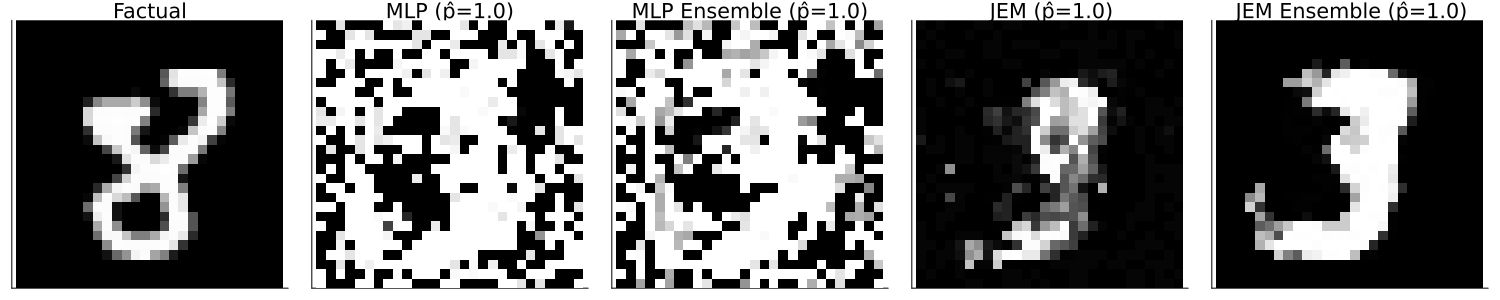
\includegraphics[width=0.8\textwidth]{../artifacts/results/images/mnist_eccco.png}
  \captionof{figure}{ECCCos for turning a 9 (nine) into a 7 (seven) for different black-box models from left to right: Multi-Layer Perceptron (a), Ensemble of MLPs (b), Joint Energy Model (c), Ensemble of JEMs (d).}\label{fig:eccco-mnist}
\end{minipage}  
\hfill
\begin{minipage}[c]{0.45\textwidth}
\captionof{algorithm}{Generating ECCCos (For more details, see Appendix~\ref{app:eccco})}\label{alg:eccco}
\begin{algorithmic}[1]
  \Require $\mathbf{x}, \mathbf{y}^+, M_{\theta}, f, \Lambda, \alpha, \mathcal{D}, T, \eta, n_{\mathcal{B}}, N_{\mathcal{B}}$ \linebreak where $M_{\theta}(\mathbf{x})\neq\mathbf{y}^+$
  \Ensure $\mathbf{x}^\prime$
  \State Initialize $\mathbf{z}^\prime \gets f^{-1}(\mathbf{x})$
  \State Generate buffer $\mathcal{B}$ of $N_{\mathcal{B}}$ conditional samples $\hat{\mathbf{x}}_{\theta}|\mathbf{y}^+$ using SGLD (Equation~\ref{eq:sgld})
  \State Run \textit{SCP} for $M_{\theta}$ using $\mathcal{D}$
  \State Initialize $t \gets 0$
  \While{\textit{not converged} or $t < T$}
  \State $\hat{\mathbf{x}}_{\theta, t} \gets \text{rand}(\mathcal{B},n_{\mathcal{B}})$
  \State $\mathbf{z}^\prime \gets \mathbf{z}^\prime - \eta \nabla_{\mathbf{z}^\prime} \mathcal{L}(\mathbf{z}^\prime,\mathbf{y}^+,\hat{\mathbf{x}}_{\theta, t}; \Lambda, \alpha)$
  \State $t \gets t+1$
  \EndWhile
  \State $\mathbf{x}^\prime \gets f(\mathbf{z}^\prime)$
\end{algorithmic}
\end{minipage}

\medskip

% \begin{minipage}[c]{\textwidth}
%   \centering
%   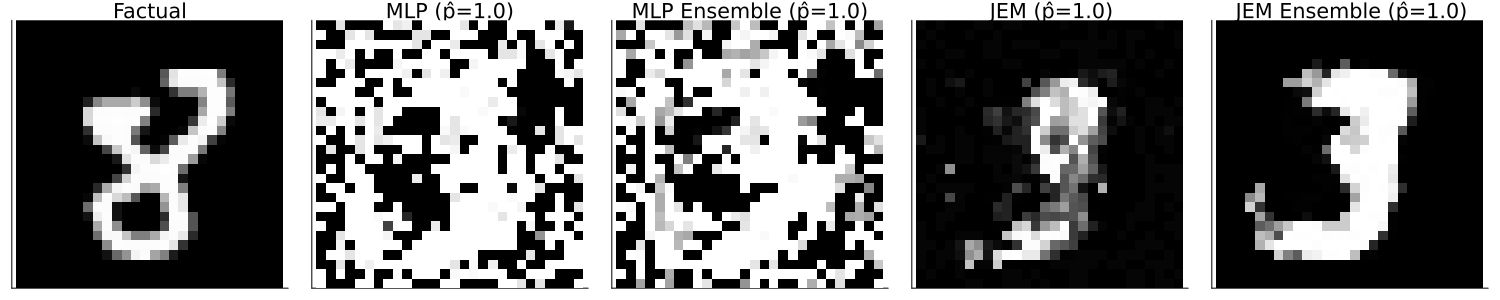
\includegraphics[width=0.8\textwidth]{../artifacts/results/images/mnist_eccco.png}
%   \captionof{figure}{Original image (left) and ECCCos for turning a 9 (nine) into a 7 (seven) for different black-box models from left to right: Multi-Layer Perceptron (MLP), Ensemble of MLPs, Joint Energy Model (JEM), Ensemble of JEMs.}\label{fig:eccco-mnist}
% \end{minipage}

\medskip

The entire procedure for Generating ECCCos is described in Algorithm~\ref{alg:eccco}. For the sake of simplicity and without loss of generality, we limit our attention to generating a single counterfactual $\mathbf{x}^\prime=f(\mathbf{z}^\prime)$ where in contrast to Equation~\ref{eq:eccco} $\mathbf{z}^\prime$ denotes a $1$-dimensional array containing a single counterfactual state. That state is initialized by passing the factual $\mathbf{x}$ through the encoder $f^{-1}$ which in our case corresponds to a simple feature transformer, rather than the encoder part of VAE as in REVISE~\citep{joshi2019realistic}. Next, we generate a buffer of $N_{\mathcal{B}}$ conditional samples $\hat{\mathbf{x}}_{\theta}|\mathbf{y}^+$ using SGLD (Equation~\ref{eq:sgld}) and conformalise the model $M_{\theta}$ through Split Conformal Prediction on training data $\mathcal{D}$.

Finally, we search counterfactuals through gradient descent. Let $\mathcal{L}(\mathbf{z}^\prime,\mathbf{y}^+,\hat{\mathbf{x}}_{\theta, t}; \Lambda, \alpha)$ denote our loss function defined in Equation~\ref{eq:eccco}. Then in each iteration, we first randomly draw $n_{\mathcal{B}}$ samples from the buffer $\mathcal{B}$ before updating the counterfactual state $\mathbf{z}^\prime$ by moving in the negative direction of that loss function. The search terminates once the convergence criterium is met or the maximum number of iterations $T$ has been exhausted. Note that the choice of convergence criterium has important implications on the final counterfactual (for more detail on this see Appendix~\ref{app:eccco}).

Figure~\ref{fig:eccco-mnist} presents ECCCos for the MNIST example from Section~\ref{background} for various black-box models of increasing complexity from left to right: a simple Multi-Layer Perceptron (MLP); an Ensemble of MLPs, each of the same architecture as the single MLP; a Joint Energy Model (JEM) based on the same MLP architecture; and finally, an Ensemble of these JEMs. Since Deep Ensembles have an improved capacity for predictive uncertainty quantification and JEMs are explicitly trained to learn plausible representations of the input data, it is intuitive to see that the plausibility of counterfactuals visibly improves from left to right. This provides some first anecdotal evidence that ECCCos achieve plausibility while maintaining faithfulness to the Black Box. 

\section{Empirical Analysis}\label{emp}

Our goal in this section is to shed light on the following research questions:

\begin{question}[Feasibility]\label{rq:feasibility}
  Is it feasible to generate plausible Counterfactual Explanations through ECCCo without relying on surrogate models?
\end{question}

\begin{question}[Drivers]\label{rq:drivers}
  Subject to feasibility, what drives the performance of ECCCo? Is it sufficient to rely on energy-based modelling to quantify the model's generative property? Is it sufficient to rely on conformal prediction to quantify the model's uncertainty?
\end{question}

We first briefly describe our experimental setup, before presenting our main results.

\subsection{Key Evaluation Metrics}\label{evaluation}

While we focus on these key evaluation metrics in the body of this paper, we also sporadically discuss outcomes with respect to other common measures used to evaluate the validity, proximity and sparsity of counterfactuals. Details can be found in Appendix~\ref{app:results}.

\subsection{Experimental Setup}

To assess and benchmark the performance of ECCCo against the state of the art, we generate multiple counterfactuals for different black-box models and datasets. In particular, we compare ECCCo to the following counterfactual generators that were introduced above: firstly; \textbf{Schut}~\citep{schut2021generating}, which minimizes predictive uncertainty; secondly, \textbf{REVISE}~\citep{joshi2019realistic}, which uses a VAE as its surrogate model; and, finally, \textbf{Wachter}~\citep{wachter2017counterfactual}, which serves as our baseline.

We use both synthetic and real-world datasets from different domains, all of which are publically available and commonly used to train and benchmark classification algorithms. The synthetic datasets include: a dataset containing two \textbf{Linearly Separable} Gaussian clusters ($n=1000$), as well as the well-known \textbf{Circles} ($n=1000$) and \textbf{Moons} ($n=2500$) data. As for real-world data, we follow~\citet{schut2021generating} and use the \textbf{MNIST}~\citep{lecun1998mnist} dataset containing images of handwritten digits such as the examples shown above. From the social sciences domain, we include Give Me Some Credit (\textbf{GMSC})~\citep{kaggle2011give}: a tabular dataset that has been studied extensively in the literature on Algorithmic Recourse~\citep{pawelczyk2021carla}. It consists of 11 numeric features that can be used to predict the binary outcome variable indicating whether or not retail borrowers experience financial distress. 

As with the example in Section~\ref{meth}, we use simple neural networks (\textbf{MLP}) and Joint Energy Models (\textbf{JEM}). For the more complex real-world datasets we also use ensembling in each case. To account for stochasticity, we generate multiple counterfactuals for each possible target class, generator, model and dataset. Specifically, we randomly sample $n^{-}$ times from the subset of individuals for which the given model predicts the non-target class $\mathbf{y}^{-}$ given the current target. We set $n^{-}=25$ for all of our synthetic datasets, $n^{-}=10$ for GMSC and $n^{-}=5$ for MNIST. Full details concerning our parameter choices, training procedures and model performance can be found in Appendix~\ref{app:setup}.

\subsection{Results}

Table~\ref{tab:results-synthetic} shows the key results for the synthetic datasets separated by model (first columns) and generator (second column). The numerical columns show the average values of our key evaluation metrics computed across all counterfactuals. Standard deviations are shown in parentheses. In bold we have highlighted the best outcome for each model and metric. To provide some sense of the statistical significance of our findings, we have added asterisks to indicate that a given value is at least one ($*$) or two ($**$) standard deviations lower than the baseline (Wachter).

Starting with the high-level results for our Linearly Separable data, we find that ECCCo produces the most faithful counterfactuals for both black-box models. This is not surprising, since ECCCo directly enforces faithfulness through regularization. Crucially though, ECCCo also produces the most plausible counterfactuals for the Joint Energy Model, which was explicitly trained to learn plausible representations of the input data. This high-level pattern is broadly consistent across all datasets and supportive of our narrative, so it is worth highlighting: ECCCos consistently achieve high faithfulness, which---subject to the quality of the model itself---coincides with high plausibility. 

Zooming in on the granular details for the Linearly Separable data, note that the list of generators in Table~\ref{tab:results-synthetic} includes `ECCCo (no CP)' and `ECCCo (no EBM)' in addition to `ECCCo' and our benchmark generators. These have been added to gain some sense of the degree to which the two components underlying ECCCo---namely energy-based modelling (EBM) and conformal prediction (CP)---drive the results. Specifically, `ECCCo (no CP)' involves no set size penalty ($\lambda_3=0$ in Equation~\ref{eq:eccco}), while `ECCCo (no EBM)' does not penalise the distance to samples generated through SGLD ($\lambda_2=0$ in Equation~\ref{eq:eccco}). The corresponding results indicate that the positive results are dominated by the effect of quantifying and leveraging the model's generative property (EBM) in our search for counterfactuals. Conformal Prediction alone only leads to marginally improved faithfulness and plausibility relative to the benchmark generators for our JEM. As a final observation for the Linearly Separable data we note that for the MLP, increased faithfulness comes at the cost of reduced plausibility. Specifically, this means that counterfactuals generated through ECCCo end up further away from individuals in the target class than those produced by our benchmark generators. 

The findings for the Moons dataset are broadly in line with the findings so far: for the JEM, ECCCo yields significantly more faithful and plausible counterfactuals than all other generators. For the MLP, faithfulness is maintained but counterfactuals are not plausible. By comparison, REVISE yields fairly plausible counterfactuals in both cases, but it does so at the cost of faithfulness. We also observe that the best results for ECCCo are achieved when using both penalties. Once again though, the generative component (EBM) has a stronger impact on the positive results for the JEM.

\import{contents/}{table-synthetic.tex}

For the Circles data, the most faithful counterfactuals are generated by ECCCo. While it appears that REVISE generates the most plausible counterfactuals in this case, we note that they are valid only half of the time (see Appendix~\ref{app:results} for a complete overview of all evaluation metrics). It turns out that in this case, the underlying VAE with default parameters has not adequately learned the data-generating process. Of course, it is possible to achieve better generative performance through hyperparameter tuning. But this example serves to illustrate that REVISE depends strictly on the quality of the surrogate model. Independent of the outcome for REVISE, however, the results do not seem to indicate that ECCCo significantly improves our plausibility metric for the Circles data. 

Moving on to our real-world datasets, the results are shown in Table~\ref{tab:results-real-world}. Once again the findings indicate that the plausibility of ECCCos is positively correlated with the capacity of the black-box model to distinguish plausible from implausible inputs. The case is very clear for MNIST: ECCCos are consistently more faithful than the corresponding counterfactuals produced by any of the benchmark generators and their plausibility gradually improves through ensembling and joint-energy modelling. For the JEM Ensemble, ECCCo is essentially on par with REVISE and does significantly better than the baseline generator. We also note that ECCCo is the only generator that consistently achieves full validity for all models (Appendix~\ref{app:results}). Interestingly, ECCCo also yields lower-cost outcomes than the baseline generator for the JEMs. 

For the tabular credit dataset (GMSC) we have struggled to get good generative and discriminative performance for our JEMs. Consequently, it is not surprising to find that ECCCo never achieves state-of-the-art plausibility, although it does improve outcomes compared to the baseline (Wachter). Concerning faithfulness, ECCCo once again consistently outperforms all other generators.

To conclude this section, we summarize our findings with reference to the opening questions. Concerning the feasibility of our proposed methodology (Research Question~\ref{rq:feasibility}), our findings demonstrate that it is indeed possible to generate plausible counterfactuals without the need for surrogate models. A related important finding is that ECCCo never sacrifices faithfulness for plausibility: any plausible ECCCo also faithfully describes model behaviour. This mitigates the risk of generating plausible explanations for models that are, in fact, highly susceptible to implausible counterfactuals as well. Our findings here indicate that ECCCo achieves this result primarily by leveraging the model's generative property. We think that further work is needed, however, to definitively answer Research Question~\ref{rq:drivers}, on which we elaborate in the following section. 

\import{contents/}{table-real-world.tex}

\section{Limitations}

Even though we have taken considerable measures to study our proposed methodology carefully, this work is limited in scope, which caveats our findings. In particular, we have found that the performance of ECCCo is sensitive to hyperparameter choices. In order to achieve faithfulness, we generally had to penalise the distance from generated samples slightly more than the distance from factual values. This choice is associated with relatively higher costs to individuals since the proposed recourses typically involve more substantial feature changes than for our benchmark generators.

Conversely, we have not found that penalising prediction set sizes disproportionately strongly had any discernable effect on our results. As discussed above, we also struggled to achieve good results by relying on conformal prediction alone. We want to caveat this finding by acknowledging that the role of CP in this context needs to be investigated more thoroughly through future work. Our suggested approach involving a smooth set size penalty may be insufficient in this context. 

The fact that our findings are primarily driven by applying ideas from energy-based modelling presents a challenge in itself: while our approach is readily applicable to models with gradient access like deep neural networks, more work is needed to generalise our methodology to other popular machine learning models such as gradient-boosted trees. Relatedly, we have encountered common challenges associated with energy-based modelling during our experiments including sensitivity to scale, training instabilities and sensitivity to hyperparameters. We have also struggled to apply our proposed approach to low-dimensional tabular data. 

\section{Conclusion}

This work leverages recent advances in energy-based modelling and conformal prediction in the context of Explainable Artificial Intelligence. We have proposed a new way to generate Counterfactual Explanations that are maximally faithful to the black-model they aim to explain. Our proposed counterfactual generator, ECCCo, produces plausible counterfactual if and only if the black-model itself has learned realistic representations of the data. This should enable researchers and practitioners to use counterfactuals in order to discern trustworthy models from unreliable ones. While the scope of this work limits its generalizability, we believe that ECCCo offers a solid baseline for future work on faithful Counterfactual Explanations.

\begin{ack}

Some of the members of TU Delft were partially funded by ICAI AI for Fintech Research, an ING — TU Delft
collaboration.

\end{ack}

\medskip

\bibliography{bib}

\appendix
\section*{Appendices}
\renewcommand{\thesubsection}{\Alph{subsection}}

\subsection{JEM}\label{app-jem}

While $\mathbf{x}_J$ is only guaranteed to distribute as $p_{\theta}(\mathbf{x}|\mathbf{y}^+)$ if $\epsilon \rightarrow 0$ and $J \rightarrow \infty$, the bias introduced for a small finite $\epsilon$ is negligible in practice~\citep{murphy2023probabilistic,grathwohl2020your}. While~\citet{grathwohl2020your} use Equation~\ref{eq:sgld} during training, we are interested in applying the conditional sampling procedure in a post-hoc fashion to any standard discriminative model. 

\subsection{Conformal Prediction}\label{app-cp}

The fact that conformal classifiers produce set-valued predictions introduces a challenge: it is not immediately obvious how to use such classifiers in the context of gradient-based counterfactual search. Put differently, it is not clear how to use prediction sets in Equation~\ref{eq:general}. Fortunately, \citet{stutz2022learning} have recently proposed a framework for Conformal Training that also hinges on differentiability. Specifically, they show how Stochastic Gradient Descent can be used to train classifiers not only for the discriminative task but also for additional objectives related to Conformal Prediction. One such objective is \textit{efficiency}: for a given target error rate $\alpha$, the efficiency of a conformal classifier improves as its average prediction set size decreases. To this end, the authors introduce a smooth set size penalty defined in Equation~\ref{eq:setsize} in the body of this paper

Formally, it is defined as $C_{\theta,\mathbf{y}}(\mathbf{x}_i;\alpha):=\sigma\left((s(\mathbf{x}_i,\mathbf{y})-\alpha) T^{-1}\right)$ for $\mathbf{y}\in\mathcal{Y}$, where $\sigma$ is the sigmoid function and $T$ is a hyper-parameter used for temperature scaling~\citep{stutz2022learning}.

Intuitively, CP works under the premise of turning heuristic notions of uncertainty into rigorous uncertainty estimates by repeatedly sifting through the data. It can be used to generate prediction intervals for regression models and prediction sets for classification models~\citep{altmeyer2022conformal}. Since the literature on CE and AR is typically concerned with classification problems, we focus on the latter. A particular variant of CP called Split Conformal Prediction (SCP) is well-suited for our purposes, because it imposes only minimal restrictions on model training. 

Specifically, SCP involves splitting the data $\mathcal{D}_n=\{(\mathbf{x}_i,\mathbf{y}_i)\}_{i=1,...,n}$ into a proper training set $\mathcal{D}_{\text{train}}$ and a calibration set $\mathcal{D}_{\text{cal}}$. The former is used to train the classifier in any conventional fashion. The latter is then used to compute so-called nonconformity scores: $\mathcal{S}=\{s(\mathbf{x}_i,\mathbf{y}_i)\}_{i \in \mathcal{D}_{\text{cal}}}$ where $s: (\mathcal{X},\mathcal{Y}) \mapsto \mathbb{R}$ is referred to as \textit{score function}. In the context of classification, a common choice for the score function is just $s_i=1-M_{\theta}(\mathbf{x}_i)[\mathbf{y}_i]$, that is one minus the softmax output corresponding to the observed label $\mathbf{y}_i$~\citep{angelopoulos2021gentle}. 

Finally, classification sets are formed as follows,

\begin{equation}\label{eq:scp}
  \begin{aligned}
    C_{\theta}(\mathbf{x}_i;\alpha)=\{\mathbf{y}: s(\mathbf{x}_i,\mathbf{y}) \le \hat{q}\}
  \end{aligned}
\end{equation}

where $\hat{q}$ denotes the $(1-\alpha)$-quantile of $\mathcal{S}$ and $\alpha$ is a predetermined error rate. As the size of the calibration set increases, the probability that the classification set $C(\mathbf{x}_{\text{test}})$ for a newly arrived sample $\mathbf{x}_{\text{test}}$ does not cover the true test label $\mathbf{y}_{\text{test}}$ approaches $\alpha$~\citep{angelopoulos2021gentle}. 

Observe from Equation~\ref{eq:scp} that Conformal Prediction works on an instance-level basis, much like Counterfactual Explanations are local. The prediction set for an individual instance $\mathbf{x}_i$ depends only on the characteristics of that sample and the specified error rate. Intuitively, the set is more likely to include multiple labels for samples that are difficult to classify, so the set size is indicative of predictive uncertainty. To see why this effect is exacerbated by small choices for $\alpha$ consider the case of $\alpha=0$, which requires that the true label is covered by the prediction set with probability equal to 1.

\subsection{Conformal Prediction}\label{app:eccco}

\subsection{Experimental Setup}\label{app:setup}
\subsection{Results}\label{app:results}

\import{contents/}{table_all.tex}


\end{document}